\section{História}

\begin{frame}
	\frametitle{Curiosidade}
	\begin{figure}[htpb]
		\centering
		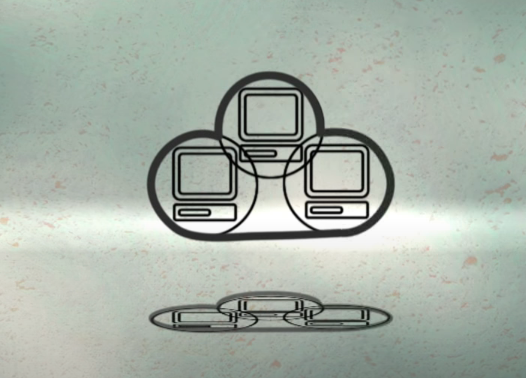
\includegraphics[width=0.6\textwidth]{server_cluster}
		\caption{A cluster of servers drawn in a system diagram \footnote{\href{https://www.youtube.com/watch?v=e3UMvBP2RRo}{Image source link}}}
	\end{figure}
\end{frame}

\subsection{Linha do tempo}

\begin{frame}
	\frametitle{Linha do tempo}
	\begin{center}
		História da computação em nuvem\cite{CCHistory}
	\end{center}
	\begin{scriptsize}
	\begin{bf}
	\begin{center}
		\begin{chronology}[10]{1955}{2010}{12cm}[\textwidth]
			\event[1955]{1965}{1955-1965}
			\event[1970]{1990}{1970-1990}
			\event[1990]{2006}{1990-2006}
			\event{2006}{2006}
			\event[2006]{2010}{2016-2010}
		\end{chronology}
	\end{center}
	\end{bf}
	\begin{itemize}
		\item (1955-1965) Problemas na infraestrutura de TI
		\item (1970-1990) Hypervisors e a internet
		\item (1990-2006) Internet para todos
		\item (2006-2006) Precipitation
		\item (2006-2010) Primeiros dias da computação em nuvem
	\end{itemize}
	\end{scriptsize}
\end{frame}

\begin{frame}
	\frametitle{Linha do tempo}
	\begin{scriptsize}
	\begin{bf}
	\begin{center}
		\begin{chronology}[10]{1955}{2010}{12cm}[\textwidth]
			\event[1955]{1965}{1955-1965}
			\event[1970]{1990}{1970-1990}
			\event[1990]{2006}{1990-2006}
			\event{2006}{2006}
			\event[2006]{2010}{2016-2010}
			\color{lightgreen}
				\event[1955]{1965}{1955-1965}
		\end{chronology}
	\end{center}
	\end{bf}
	\end{scriptsize}
	\begin{center}
		(1955-1965)

		Problemas na infraestrutura de TI
	\end{center}
\end{frame}

\begin{frame}
	\frametitle{(1955-1965) Problemas na infraestrutura de TI}
	\begin{itemize}
		\item 1942 - John Vincent Atanasoff construiu o computador ABC
		\item Server/Mainframe (Componentes principais):
			\begin{itemize}
				\item Uma CPU
				\item Um dispositivo de armazenamento de dados
			\end{itemize}
		\item 1960 - Muito caro para aderir os computadores
			\begin{itemize}
				\item Sala inteira para o servidor (Manter temperatura ideal, espaço, etc\dots)
				\item Computador
				\item Funcionários especializados
				\item Problemas para adaptar o software
			\end{itemize}
	\end{itemize}
\end{frame}

\begin{frame}
	\frametitle{(1955-1965) Problemas na infraestrutura de TI}
	\begin{itemize}
		\item Apenas empresas que com poder aquisitivo conseguiram aderir os computadores
		\item 1961 - John MacCharty fez uma palestra no MIT
			\begin{itemize}
				\item Computação poderia ser vendida como água ou eletricidade \cite{SimsonTCI}
				\item Mas seria necessário de uma grande evolução tecnológica
			\end{itemize}
	\end{itemize}
\end{frame}

\begin{frame}
	\frametitle{Linha do tempo}
	\begin{scriptsize}
	\begin{bf}
	\begin{center}
		\begin{chronology}[10]{1955}{2010}{12cm}[\textwidth]
			\event[1955]{1965}{1955-1965} \event[1970]{1990}{1970-1990}
			\event[1990]{2006}{1990-2006}
			\event{2006}{2006}
			\event[2006]{2010}{2016-2010}
			\color{lightgreen}
				\event[1970]{1990}{1970-1990}
		\end{chronology}
	\end{center}
	\end{bf}
	\end{scriptsize}
	\begin{center}
		(1970-1990) Hypervisors e a internet
	\end{center}
\end{frame}

\begin{frame}
	\frametitle{(1970-1990) Hypervisors e a internet}
	\begin{itemize}
		\item Diminiur os custos da adoção do computador
			\begin{itemize}
				\item Múltiplos usuários podem compartilhar o mesmo armazenamento e o poder de processamento da CPU
			\end{itemize}
		\item 1970 - Nasceu a tecnologia da virtualização
			\begin{itemize}
				\item Um computador pode ser particionado em vários partes
				\item Cada parte pode rodar um código independente
				\item Cada parte é chamada de Máquina Virtual (VM)
				\item O server principal é chamado de \it{host}
			\end{itemize}
		\item O server tem um software que cria roda essas VMs virtualmente compartilhando seus recursos, dessa forma a máquina física se torna um hypervisor
	\end{itemize}
\end{frame}

\begin{frame}
	\frametitle{(1970-1990) Hypervisors e a internet}
	\begin{itemize}
		\item 1983 - A internet nasceu
			\begin{itemize}
				\item Começou pelo projeto ARPANet para comunicação de professores de universidades
			\end{itemize}
		\item Foi introduzida a arquitetura cliente-servidor, o cliente e o server eram os mainframes interagindo com código e informação conectados por cabos (Internet)
		\item Conforme os números de páginas foram crescendo o número de servers cresceram
			\begin{itemize}
				\item Os servers se moveram para datacenters
			\end{itemize}
	\end{itemize}
\end{frame}

\begin{frame}
	\frametitle{Linha do tempo}
	\begin{scriptsize}
	\begin{bf}
	\begin{center}
		\begin{chronology}[10]{1955}{2010}{12cm}[\textwidth]
			\event[1955]{1965}{1955-1965}
			\event[1970]{1990}{1970-1990}
			\event[1990]{2006}{1990-2006}
			\event{2006}{2006}
			\event[2006]{2010}{2016-2010}
			\color{lightgreen}
				\event[1990]{2006}{1990-2006}
		\end{chronology}
	\end{center}
	\end{bf}
	\end{scriptsize}
	\begin{center}
		(1990-2006) Internet para todos
	\end{center}
\end{frame}

\begin{frame}
	\frametitle{(1990-2006) Internet para todos}
	\begin{itemize}
		\item A empresas maiores precisavam de datacenters maiores
		\item Problemas:
			\begin{itemize}
				\item If your website was not accessed much, all the hardware hosting your code and everything that comes with it would be unused. This would lead to software providers  bleeding capital by keeping the servers on.
				\item "Scaling" business for a software company was difficult as it required managing physical devices and real estate space. Consider facebook.com, a website with an incredible growth rate. Keeping up with that growth would be impossible, causing the website to crash (the case of Facebook's predecessor - Facesmash, the local intranet of Harvard university).
				\item The speed of shipping updates was a problem since developers had to manually upload the code on the host server each time, to maintain its health and performance. Some days it would even involve marching into the data center with a screwdriver to repair broken software that was being served.
				\item Lastly, the user experience (UX) was worsening. The closer the location of the person requesting the website to the location of the servers, the faster the website loads for them. This is a case in point for early users of google.com, where servers were hosted in the USA. A user accessing the website from the USA would have a seamless experience, but someone accessing it from India would get frustrated with page-load times.
			\end{itemize}
		\item In a nutshell, physical machine management, the cost of handling useless machines, and scaling are the top 3 problems internet-based companies faced. Back then, the droplets of technology started coming together just as water vapor in the cloud condenses into water drops. And then, the cloud burst.
	\end{itemize}
\end{frame}

\begin{frame}
	\frametitle{Linha do tempo}
	\begin{scriptsize}
	\begin{bf}
	\begin{center}
		\begin{chronology}[10]{1955}{2010}{12cm}[\textwidth]
			\event[1955]{1965}{1955-1965}
			\event[1970]{1990}{1970-1990}
			\event[1990]{2006}{1990-2006}
			\event{2006}{2006}
			\event[2006]{2010}{2016-2010}
			\color{lightgreen}
				\event{2006}{2006}
		\end{chronology}
	\end{center}
	\end{bf}
	\end{scriptsize}
	\begin{center}
		(2006) Precipitation
	\end{center}
\end{frame}

\begin{frame}
	\frametitle{(2006) Precipitação}
	\begin{itemize}
		\item Grandes empresas (\it{Google, Amazon, eBay, etc\dots})
			\begin{itemize}
				\item Também tiveram problemas, mas eles tinham dinheiro
				\item Criaram \it{data centers} com centenas/milhares de servers de alta qualidade no mundo inteiro
				\item Até mesmo eles tinham máquinas ociosas fora da temporada que só traziam prejuízos
				\item Decidiram começar a alugar essas máquinas
			\end{itemize}
		\item 03/03/2006 - "Cloud Computing" foi introduzino no mundo como forma de aluguel de poder computacional
		\item A Amazon chamou essa difisão de Amazon Web Services (AWS)
		\item A AWS foi a primeira de muitos provedores de cloud
		\item Dessa forma empresas não precisam mais gerenciar sua própria infraestrutura de TI em data centers
		\item Depois de 50 anos o sonho de John McCharty foi realizado
	\end{itemize}
\end{frame}

\begin{frame}
	\frametitle{Linha do tempo}
	\begin{scriptsize}
	\begin{bf}
	\begin{center}
		\begin{chronology}[10]{1955}{2010}{12cm}[\textwidth]
			\event[1955]{1965}{1955-1965}
			\event[1970]{1990}{1970-1990}
			\event[1990]{2006}{1990-2006}
			\event{2006}{2006}
			\event[2006]{2010}{2016-2010}
			\color{lightgreen}
				\event[2006]{2010}{2016-2010}
		\end{chronology}
	\end{center}
	\end{bf}
	\end{scriptsize}
	\begin{center}
		(2006-2010) Primeiros dias da computação em nuvem
	\end{center}
\end{frame}

\begin{frame}
	\frametitle{(2006-2010) Primeiros dias da computação em nuvem}
	\begin{itemize}
		\item Por 6 anos a AWS não teve competição e consegui estabelecer seu monopólio na área de nuvem
		\item A computação em nuvem permitiu que a empresa possa focar no desenvolvimento e deixar a parte da infra estrutura para a computação em nuvem
			\begin{itemize}
				\item Os dados são criptografados e seguros
				\item Dados são armazenados com redundância em nuvem
				\item Escalabilidade
				\item De fácil deploy
				\item Alta disponibilidade
			\end{itemize}
	\end{itemize}
\end{frame}

\begin{frame}
	\frametitle{(2006-2010) Primeiros dias da computação em nuvem}
	\begin{figure}[htpb]
	\begin{center}
	\begin{tiny}
	\begin{tikzpicture}[scale=1, transform shape]
		\node (A) at (0,4) {\normalsize On-Site};
		\node (A1) at ($(A) - (0,0.6)$)  [draw,thick,minimum width=75,minimum height=15] {Applicação};
		\node (A2) at ($(A1) - (0,0.6)$) [draw,thick,minimum width=75,minimum height=15] {Data};
		\node (A3) at ($(A2) - (0,0.6)$) [draw,thick,minimum width=75,minimum height=15] {Runtime};
		\node (A4) at ($(A3) - (0,0.6)$) [draw,thick,minimum width=75,minimum height=15] {Middleware};
		\node (A5) at ($(A4) - (0,0.6)$) [draw,thick,minimum width=75,minimum height=15] {O/S};
		\node (A6) at ($(A5) - (0,0.6)$) [draw,thick,minimum width=75,minimum height=15] {Virtualization};
		\node (A7) at ($(A6) - (0,0.6)$) [draw,thick,minimum width=75,minimum height=15] {Servers};
		\node (A8) at ($(A7) - (0,0.6)$) [draw,thick,minimum width=75,minimum height=15] {Storage};
		\node (A9) at ($(A8) - (0,0.6)$) [draw,thick,minimum width=75,minimum height=15] {Networking};
		\node (B) at (3,4) {\normalsize IaaS};
		\node (B1) at ($(B) - (0,0.6)$)  [draw,thick,minimum width=75,minimum height=15] {Applicação};
		\node (B2) at ($(B1) - (0,0.6)$) [draw,thick,minimum width=75,minimum height=15] {Data};
		\node (B3) at ($(B2) - (0,0.6)$) [draw,thick,minimum width=75,minimum height=15] {Runtime};
		\node (B4) at ($(B3) - (0,0.6)$) [draw,thick,minimum width=75,minimum height=15] {Middleware};
		\node (B5) at ($(B4) - (0,0.6)$) [draw,thick,minimum width=75,minimum height=15] {O/S};
		\node (B6) at ($(B5) - (0,0.6)$) [lightgreen,draw,thick,minimum width=75,minimum height=15] {Virtualization};
		\node (B7) at ($(B6) - (0,0.6)$) [lightgreen,draw,thick,minimum width=75,minimum height=15] {Servers};
		\node (B8) at ($(B7) - (0,0.6)$) [lightgreen,draw,thick,minimum width=75,minimum height=15] {Storage};
		\node (B9) at ($(B8) - (0,0.6)$) [lightgreen,draw,thick,minimum width=75,minimum height=15] {Networking};
		\node (C) at (6,4) {\normalsize PaaS};
		\node (C1) at ($(C) - (0,0.6)$)  [draw,thick,minimum width=75,minimum height=15] {Applicação};
		\node (C2) at ($(C1) - (0,0.6)$) [draw,thick,minimum width=75,minimum height=15] {Data};
		\node (C3) at ($(C2) - (0,0.6)$) [lightgreen,draw,thick,minimum width=75,minimum height=15] {Runtime};
		\node (C4) at ($(C3) - (0,0.6)$) [lightgreen,draw,thick,minimum width=75,minimum height=15] {Middleware};
		\node (C5) at ($(C4) - (0,0.6)$) [lightgreen,draw,thick,minimum width=75,minimum height=15] {O/S};
		\node (C6) at ($(C5) - (0,0.6)$) [lightgreen,draw,thick,minimum width=75,minimum height=15] {Virtualization};
		\node (C7) at ($(C6) - (0,0.6)$) [lightgreen,draw,thick,minimum width=75,minimum height=15] {Servers};
		\node (C8) at ($(C7) - (0,0.6)$) [lightgreen,draw,thick,minimum width=75,minimum height=15] {Storage};
		\node (C9) at ($(C8) - (0,0.6)$) [lightgreen,draw,thick,minimum width=75,minimum height=15] {Networking};
		\node (D) at (9,4) {\normalsize SaaS};
		\node (D1) at ($(D) - (0,0.6)$)  [lightgreen,draw,thick,minimum width=75,minimum height=15] {Applicação};
		\node (D2) at ($(D1) - (0,0.6)$) [lightgreen,draw,thick,minimum width=75,minimum height=15] {Data};
		\node (D3) at ($(D2) - (0,0.6)$) [lightgreen,draw,thick,minimum width=75,minimum height=15] {Runtime};
		\node (D4) at ($(D3) - (0,0.6)$) [lightgreen,draw,thick,minimum width=75,minimum height=15] {Middleware};
		\node (D5) at ($(D4) - (0,0.6)$) [lightgreen,draw,thick,minimum width=75,minimum height=15] {O/S};
		\node (D6) at ($(D5) - (0,0.6)$) [lightgreen,draw,thick,minimum width=75,minimum height=15] {Virtualization};
		\node (D7) at ($(D6) - (0,0.6)$) [lightgreen,draw,thick,minimum width=75,minimum height=15] {Servers};
		\node (D8) at ($(D7) - (0,0.6)$) [lightgreen,draw,thick,minimum width=75,minimum height=15] {Storage};
		\node (D9) at ($(D8) - (0,0.6)$) [lightgreen,draw,thick,minimum width=75,minimum height=15] {Networking};
	\end{tikzpicture}
	\end{tiny}
	\end{center}
	\caption{Imagem retirado do site da redhat\footnote{\href{https://www.redhat.com/cms/managed-files/iaas-paas-saas-diagram5.1-1638x1046.png}{RedHat IaaS, PaaS e SaaS}}}
	\end{figure}
\end{frame}
